\documentclass[aps,prl,twocolumn,superscriptaddress]{revtex4-1}

\bibliographystyle{apsrev4-1}

\usepackage{fancyhdr} %for the header

\usepackage{hyperref} %hyperlinked references

%%%%%%%%%%%%%%%%%%% PACKAGES %%%%%%%%%%%%%%%%%%%%%%%
\usepackage{verbatim} %for multi-line comments \begin{comment}
\usepackage{amsmath} %ams math
\usepackage{amsthm} % Theorem Formatting
\usepackage{amssymb}	% Math symbols such as \mathbb
\usepackage{graphicx} % Allows for eps images
%\usepackage{multicol} % Allows for multiple columns
\usepackage[dvips,letterpaper,margin=0.75in,bottom=0.5in]{geometry}
 % Sets margins and page size
\makeatletter % Need for anything that contains an @ command 
\makeatother % End of region containing @ commands
\renewcommand{\labelenumi}{\Bigg(\alph{enumi}\Bigg)} % Use letters for enumerate

\let\baraccent=\= % rename builtin command \= to \baraccent
\renewcommand{\=}[1]{\stackrel{#1}{=}} % for putting numbers above =

\newcommand{\gae}{\lower 2pt \hbox{$\,
    \buildrel{\scriptstyle >}\over {\scriptstyle \sim}\,$}}
\newcommand{\lae}{\lower 2pt \hbox{$\,
    \buildrel{\scriptstyle <}\over {\scriptstyle \sim}\,$}}

\newcommand{\R}{\mathbb{R}}
\newcommand{\diag}{\mathrm{diag}}

\newcommand{\Tr}{\mathrm{Tr}}
\newcommand{\abs}[1]{\left| #1 \right|} % for absolute value
\newcommand{\avg}[1]{\left< #1 \right>} % for average
\let\underdot=\d % rename builtin command \d{} to \underdot{}
\renewcommand{\d}[2]{\frac{d #1}{d #2}} % for derivatives
\newcommand{\dd}[2]{\frac{d^2 #1}{d #2^2}} % for double derivatives
\newcommand{\pd}[2]{\frac{\partial #1}{\partial #2}} 
% for partial derivatives (long form)
\newcommand{\spd}[2]{\partial_{#2}{#1}}  %for partial derivatives (short form)
\newcommand{\pdd}[2]{\frac{\partial^2 #1}{\partial #2^2}} 
% for double partial derivatives
\newcommand{\pdc}[3]{\left\Bigg( \frac{\partial #1}{\partial #2}
	\right\Bigg)_{#3}} % for thermodynamic partial derivatives
\newcommand{\ket}[1]{\big| #1 \big\rangle} % for Dirac bras
\newcommand{\bra}[1]{\big\langle #1 \big|} % for Dirac kets
\newcommand{\braket}[2]{\big\langle #1 \vphantom{#2} \big|
	#2 \vphantom{#1} \big\rangle} % for Dirac brackets
\newcommand{\sbraket}[1]{\big\langle #1 \vphantom{#1} \big|
	#1 \vphantom{#1} \big\rangle} % for Dirac brackets with same bra as ket
\newcommand{\matrixel}[3]{\big\langle #1 \vphantom{#2#3} \big|
	#2 \big| #3 \vphantom{#1#2} \big\rangle} % for Dirac matrix elements
\newcommand{\smatrixel}[2]{\big\langle #1 \vphantom{#1#2} \big|
	#2 \big| #1 \vphantom{#2#1} \big\rangle} % for Dirac matrix elements with same bra as ket
\newcommand{\proj}[1]{\ket{#1}\bra{#1}}
\newcommand{\redmatrixel}[3]{\langle #1 \big\|#2 \big\| #3\rangle}
\DeclareMathOperator{\Pf}{Pf}

%\newcommand{\id}{\mathbb{1}} 

\let\adot=\dot %dots above things (derivative sign)
\renewcommand{\dot}[2]{\v{#1}\cdot \v{#2}} %dot product of two vectors
\newcommand{\cross}[2]{\v{#1}\times \v{#2}} %cross product of two vectors

\newcommand{\eps}{\varepsilon} %squiggly epsilon
\providecommand{\cc}{\ensuremath{\mathrm{cm}^3}}
\providecommand{\e}[1]{\ensuremath{\times 10^{#1}}} %For scientific notation

%%%%%%% markup
\usepackage{color}
\usepackage{ulem}
\newcommand{\Romain}[1]{{\color{red} (Romain) #1}}
\newcommand{\Mike}[1]{{\color{blue} (Mike) #1}}
\newcommand{\Mikedel}[1]{{\color{blue} \sout{#1}}}
\newcommand{\Will}[1]{{\color{green} (Will) #1}}
\newcommand{\Joel}[1]{{\color{magenta} (Joel) #1}}

%%%%%% Use the following commands to erase comments
%% \renewcommand{\Romain}[1]{}
%% \renewcommand{\Mike}[1]{}
%% \renewcommand{\Mikedel}[1]{}
%% \renewcommand{\Will}[1]{}
%% \renewcommand{\Joel}[1]{}

\begin{document}

\title{Data 200C: Graduate Project Report}

\author{William Berdanier}
%\email[]{wberdanier@berkeley.edu}
\affiliation{Department of Physics, University of California, Berkeley, CA 94720, USA}

\author{Illan Halpern}
%\email[]{illan@berkeley.edu}
\affiliation{Department of Physics, University of California, Berkeley, CA 94720, USA}

\date{\today}

%\begin{abstract}
%Abstract.
%\end{abstract}

\maketitle

In this project, we sought to classify a bundle of unlabeled images into one of 20 categories using the techniques of data science on a  larger bundle of labeled training images. We first loaded and cleaned our images, then performed exploratory data analysis to find distinguishing features. We then fit four models to the data, optimizing each (and doing more EDA as needed), then finally output our test predictions for our best-performing model. 

\section{Exploratory Data Analysis}

We began our exploratory data analysis by picking a suitable visualization method. Since our features were scalar numbers and we wanted to easily see differences across 20 categories, we decided that a bar plot would best display the variations. In general, a good feature should vary strongly across the various categories. We began by inspecting the required features, namely image size, aspect ratio, and the average value of the red channel. Image size in particular was very distinguishing, though marred by the large variance in the image sizes within a category (such as `bear'). We also discovered a few issues with the data: (1) some of the data was actually uncleaned (for instance, \texttt{bear\_00012.jpg} was actually a `teddy-bear'), and (2) some of the images were in grayscale. After moving a few images to their correct folders, we then split our training data into color images and gray images. Since there were only 12 gray images out of 1500, we decided to exclude them from EDA.

We then brainstormed possible types of distinguishing features, browsing through the documentation of  \texttt{skimage.feature} and using our domain knowledge of the images. We posited that (1) color and (2) shape (corners, edges, etc.) would be useful types of features. We immediately decided to use the average of the blue and green channels as features to complement the average of the red channel. We then postulated that looking at other color spaces would be useful. We explored casting the images into the HSV (Hue-Saturation-Value) color space and looking at the average of the Hue, Saturation and Value (`brightness') channels. This provided a nice complement to the RGB channels, since, for instance, the Value channel corresponded to brightness, and we would expect e.g. gorillas to be dark while airplanes would be bright. We further added a decomposition into the XYZ color space, which is a color space that tries to more closely model human perception, such that a 1\% difference in X, Y or Z corresponds to a 1\% `visual difference' (see \texttt{GradProject\_NB2.ipynb} for a list of sources). 

\begin{figure}
	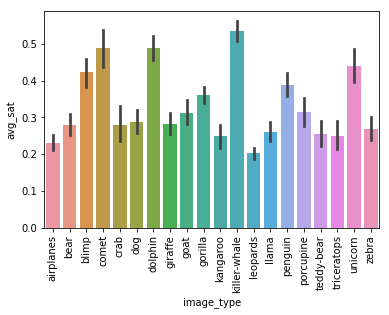
\includegraphics[width = 0.49\columnwidth]{avg_sat.png}
	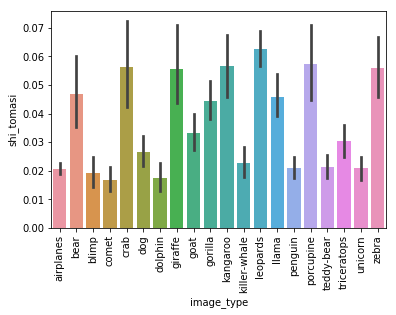
\includegraphics[width = 0.49\columnwidth]{shi_tomasi.png}
	\caption{\label{fig:EDA} Left: average of the Saturation channel (HSV color space). Right: Mean of the Shi-Tomasi corner-finding matrix on the training images. These are good features because they clearly distinguish certain (non-strongly overlapping) categories.}
\end{figure}

\begin{figure}
	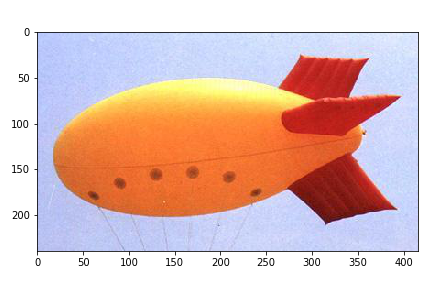
\includegraphics[width = 0.45\columnwidth]{test_image.png}
	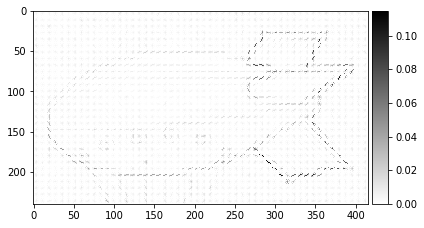
\includegraphics[width = 0.48\columnwidth]{test_image_HOG.png}
	\caption{\label{fig:HOG} Histogram of Oriented Gradients applied to a test image. The HOG algorithm detects sharp edges in images and is thus useful for classifying images with sharp features.}
\end{figure}

We then tried to get more creative with the color features. We quickly realized that `average color' would not be particularly representative of the actual colors in the image: for instance, an image with equal parts in several colors could have an average of brown, even if there was no brown in the image. Instead, we implemented a method to find the dominant color in an image using K-means clustering (\texttt{scikit-learn.KMeans}) on the RGB information. This nicely extracted the largest cluster in colorspace for each image's pixels, and visually matched the observed `dominant color'. However, this feature sadly did not end up contributing much. It was both very time-intensive to compute, taking by far the longest among all our features, and also gave us very little new information: the bar plots for this feature (R,G,B of the dominant color) picked out the same categories as the simple average of the color channels. One other feature that did not pan out was the cross-correlation among the RGB color channels; unfortunately, this feature did not vary much among categories. We did not include either in our final model.

We next moved on to including some measure of how many corners and edges an image had, which we would expect to distinguish categories like zebras and porcupines. We tried most of the algorithms for finding corners and edges that were built into \texttt{skimage}, including the Harris, matrix of Hessian determinants, and Shi-Tomasi corner finding algorithms. These algorithms produced a matrix output with the same size as the input image, which naturally led to considering quantities like the mean, median, and max of the matrix (since we needed to extract a scalar). We tried these in turn; the mean of the Shi-Tomasi matrix was especially good at picking out the categories with spines, stripes and spots (Fig.~\ref{fig:EDA}). One other intriguing feature we found was the maximal value of the Histogram of Oriented Gradients, which roughly corresponds to the `sharpest corner' in an image (the HOG itself counts occurrences of gradient orientation in localized portions of an image). This feature can be visualized as in Fig.~\ref{fig:HOG}, showing the edges of the various parts of the blimp and their sharpness.


\section{Model-Fitting}

\begin{figure}
	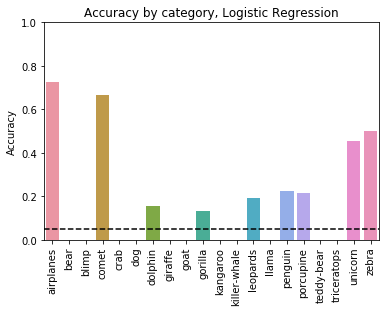
\includegraphics[width = 0.49\columnwidth]{logreg.png}
	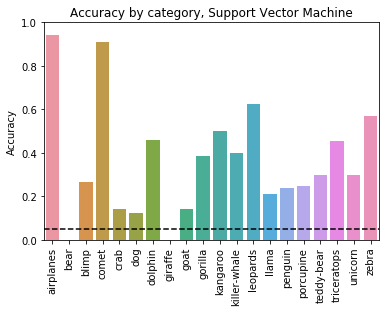
\includegraphics[width = 0.49\columnwidth]{SVM.png}
	\caption{\label{fig:models} Comparison of the accuracy of logistic regression (25\%) with SVM (40\%). Dashed black line is random guessing (5\%).}
\end{figure}


We explored 4 classes of classification models to train the data and make predictions. Below we go over them, one by one, discussing hyper-parameter choices and summarizing results. Finally, we contrast and compare results from these models. For all of them, we used only 80\% of the training data to train, while keeping the remaining 20\% to be used as a validation set. All of the below accuracies are for color images; we separately trained each model on gray images using the (much smaller) gray feature set. We trained on the gray versions of \textit{all} images by casting the color images to gray, to get more data than the 12 initially gray images.

\paragraph{Logistic Regression.} To perform the logistic regression, we used the method \texttt{LogisticRegressionCV} from  \texttt{sklearn.linear\_model}. This method uses cross validation (with the default being 5-fold on v0.22) on a logistic regression mode to find an optimal value of the regularization parameter $\alpha.$  It can be used with either L1 or L2 regularization functions, but defaults to L2. With this model, both train accuracy and validation accuracy achieved were around 24\%.

\paragraph{K-Nearest Neighbors.} We implemented K-Nearest neighbors using the method \texttt{KNeighborsClassifier} from \texttt{sklearn.neighbors}. To create the model, we had to choose both the number of neighbors and whether they were to be weighted uniformly or with weights going as the inverse of the  distance. In the latter case, we could choose to measure the distance using the $L^p$ metric for any positive integer $p$ ($p=1$ corresponding to Manhattan distance and $p=2$ corresponding to the usual Euclidian distance).

In order for distance to be a meaningful measure, and not wrongly overweight certain features, we first normalized all our features to have mean zero and variance 1 before inputting them into the K-nearest Neighbors model. We also performed a search over parameter space using \texttt{GridSearchCV} and found the optimal parameters to be about $15$ neighbors and $p=1.$ Our best K-Nearest Neighbors model achieved an accuracy of 100\% on the training set and 33.6\% on the validation set.


\paragraph{Random Forest.} Our Random Forest (RF) model, implemented with the method \texttt{RandomForestClassifier} from \texttt{sklearn.ensemble}, running on default settings was able to achieve a training accuracy of over 99\% and a validation accuracy of about 35\%. We optimized this with \texttt{GridSearchCV} to 38.2\% using 9 max features per split, 10 minimum samples per leaf, and 200 estimators; normalization was not needed since the RF does not compute and compare distances between features. 

\paragraph{Support Vector Machine.} Our Support Vector Machine (SVM) model was implemented with \texttt{sklearn.svm.SVC}. Here again it is important to normalize the data for the same reason we did for K-Nearest neighbors: distances are used (in the present case, Euclidean distance). Important choices that need to be made in selecting such a model are  the penalty parameter $C$ and the kernel to be used. Using \texttt{GridSearchCV} to optimize over these choices, we were able to obtain a train accuracy of about $64.7\%$ with a validation accuracy of about $40.1\%$.

\subsection{Comparison of Results and Conclusion}

As measured by their validation accuracy, the models studied got increasingly better in the order presented. Comparing validation and test accuracies seems to indicate that the Logistic Regression model was underfitting (large bias, low variance) while the Random Forest model was overfitting (low bias, high variance). The SVM and RF models were comparable in performance and outperformed both the logistic regression and K-Nearest Neighbors models (see e.g. Fig.~\ref{fig:models}). 

In conclusion, this was a valuable experience with using the techniques of data science on a real problem. Image recognition is clearly very hard, and finding insightful features, even without the limitations of only using scalar features, is a considerable challenge. We also implemented a neural network using \texttt{pytorch}; it is somewhat depressing that all of our modelling is quickly matched by even a simple neural network (LeNet). 


%
%\bibliography{report}
%\bibliographystyle{apsrev4-1}



\end{document}
